\documentclass[runningheads]{llncs}
% Add PDF bookmarks and metadata
\usepackage[bookmarksopen,
bookmarksopenlevel=1,
bookmarksdepth=2
pdftex,
pdfauthor={Tim Kräuter},
pdftitle={A feature-based taxonomy of coordination approaches},
pdfsubject={Classification and comparison of coordination approaches},
pdfkeywords={Coordination language, ADL, Coordination framework, Feature model, Taxonomy}
]{hyperref}
%
\usepackage{graphicx}
% to display URLs in blue roman font according to Springer's eBook style:
% \renewcommand\UrlFont{\color{blue}\rmfamily}

\usepackage{orcidlink} % Orcid links
% Fix underscore in dois
\usepackage[strings]{underscore}
% Modern tables
\usepackage{tabularray}
% Diagonal lines
\UseTblrLibrary{diagbox}
% Quote command
\newcommand{\quotes}[1]{``#1''}
% Feature command
\newcommand{\feature}[1]{\vskip 0.5em \textbf{#1}}

% proposed changes commands
\usepackage{color}
\usepackage{todonotes}
\usepackage[normalem]{ulem}
\definecolor{mygreen}{rgb}{0.0, 0.66, 0.35}
\newcommand{\jdChange}[2]{{\color{green!20}JD:} {\color{gray}\sout{#1}} {\color{mygreen}{#2}}}


\begin{document}

\title{A feature-based taxonomy of coordination approaches}

\author{Tim Kr\"{a}uter\inst{1}\orcidlink{0000-0003-1795-0611} \and
Julien Deantoni\inst{2}\orcidlink{0000-0001-6962-7846}
Adrian Rutle\inst{1}\orcidlink{0000-0002-4158-1644} \and
Harald K\"{o}nig\inst{3,1}\orcidlink{0000-0001-6304-6311} \and
Yngve Lamo\inst{1}\orcidlink{0000-0001-9196-1779}}
%
\authorrunning{T. Kräuter et al.}
\institute{Western Norway University of Applied Sciences, Bergen, Norway  \\
\email{tkra@hvl.no, aru@hvl.no, yla@hvl.no} \and
University Cote d’Azur, Sophia Antipolis, France \\
\email{julien.deantoni@univ-cotedazur.fr} \and
University of Applied Sciences, FHDW, Hanover, Germany\\
\email{harald.koenig@fhdw.de}}
%
\maketitle

\begin{abstract}

Complex domains necessitate the utilization of multiple interacting software systems.
Various categories of coordination approaches, such as coordination languages, co-simulation approaches, architecture description languages, and coordination frameworks, have been proposed to ensure seamless integration of these systems.
In this paper, we present a comprehensive feature-based taxonomy of these categories, which have previously only been studied in isolation.
The taxonomy uncovers common and unique features across the coordination approaches.
It can be used to make informed decisions about the choice of coordination approaches for specific use cases.

\end{abstract}

\keywords{
	Co-simulation \and
	Coordination language \and
	ADL \and
	Coordination framework \and
	Taxonomy \and
	Feature model
}

\section{Introduction} \label{sec: introduction}
Complex domains require multiple interacting software systems to meet their demands. 
Coordination approaches are necessary to ensure the effective integration of these systems.
The study of coordination approaches appears to be fragmented, with disparate investigations conducted on different abstraction levels, pursuing varied goals, and utilizing diverse terminology, resulting in different categories of approaches, namely \textit{coordination languages} (\cite{papadopoulosCoordinationModelsLanguages1998}), \textit{Co-simulation approaches} (\cite{gomesCoSimulationSurvey2019}), \textit{architecture description languages} (\cite{clementsSurveyArchitectureDescription1996}), and \textit{coordination frameworks} (\cite{krauterBehavioralConsistencyMultimodeling2023,varalarsenBehavioralCoordinationOperator2015}).
% Motivation
To the best of our knowledge, evaluations of coordination approaches have been limited to their respective communities.
This isolation hinders a comprehensive understanding of coordinating software systems, leading to the development of the same features independently with limited reuse.

% Contribution and outline
First, we introduce the different categories of coordination approaches to paint a picture of the different communities (\autoref{sec: approaches}) and discuss our methodology in \autoref{sec: methodology}.
Our main contribution is a comprehensive taxonomy, represented as a \textit{feature model}~\cite{kangFeatureOrientedDomainAnalysis1990} to categorize coordination approaches within a unified framework ((\autoref{sec: taxonomy})).
The taxonomy allows the comparison of coordination approaches across the different categories.
Moreover, we apply the taxonomy to evaluate 17 distinct approaches spanning the aforementioned categories (\autoref{sec: application}) and publish our findings in a public dataset~\cite{timkrauterArtifactsCoordination2024}.
Finally, we discuss our findings in \autoref{sec: findings} before concluding in \autoref{sec: conclusion}, meaning we identify the typical features for each category, provide general insights, and cluster the approaches regarding their similarity.

\section{Categories of coordination approaches} \label{sec: approaches}

\autoref{fig: overview} gives an overview of the different categories of coordination approaches.
The categories of coordination approaches broadly operate on different abstraction levels, namely the \textit{execution}, \textit{model}, and \textit{language} levels.
We will explain each abstraction level and the accompanying coordination approaches from the bottom up.
A detailed explanation of each category is given in the following subsections.
In general, the right abstraction level to address coordination depends on the specific use case and goals at hand, meaning approaches on each abstraction level have their advantages and disadvantages.

\begin{figure}[ht]
	\centering
	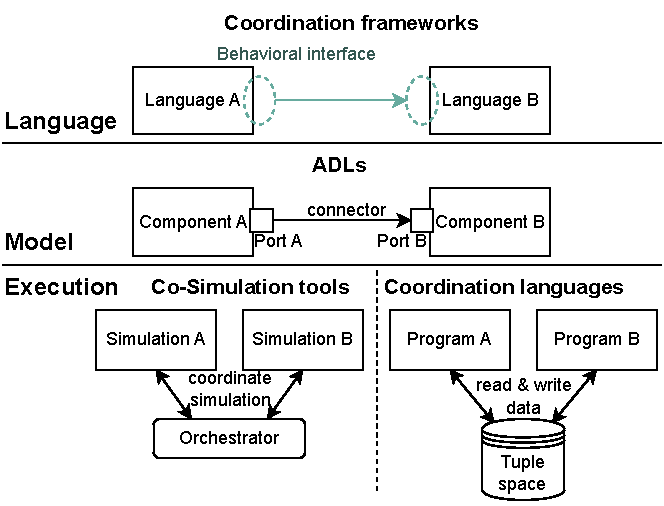
\includegraphics[width=1\textwidth]{images/overview}
	\caption{Overview of coordination approaches}
	\label{fig: overview}
\end{figure}

% Execution level
\textbf{Execution level:} Approaches on the \textit{execution level} aim to deal with coordination by interfacing directly with executable binaries or source code.
We identified two distinct categories on this level: co-simulation approaches and coordination languages.
Such approaches are overviewed in \autoref{subsec: cosim} and \autoref{subsec: coordlang}.

% Model level
\textbf{Model level:}
\textit{Architecture Description Languages (ADLs)} operate on the \textit{model} level, i.e., each \textit{component} is given by a behavioral model, for example, a process algebra.
An overview of ADLs is given in \autoref{subsec: adl}.

% Language level
\textbf{Language level:}
\textit{Coordination frameworks} operate on the language level since they allow coordination of models conforming to \textit{different} behavioral languages.
They are outlined in \autoref{subsec: frameworks}.

\subsection{Co-simulation approaches} \label{subsec: cosim}

% General description
\textit{Co-simulation approaches} involve coordinating timely exchanges of information between multiple simulations running concurrently. In this configuration, a simulation is the execution of a simulation unit that consumes inputs and produces outputs. A simulation unit is typically specified as a \textit{black box}, meaning its behavior is opaque and accessible only through its simulation interface.
Using such interfaces, the co-simulation must ensure the temporal and causal relationships between each simulation. This is usually achieved by defining an \textit{orchestrator}~\cite{gomesCoSimulationSurvey2019}, which dictates the progression of simulated time and transfers data between simulations.
Co-simulation approaches are categorized as \textit{Discrete Event} (DE), \textit{Continuous Time} (CT), or \textit{Hybrid} if DE and CT aspects are mixed~\cite{gomesCoSimulationSurvey2019}.

% Standards
Currently, there are two main standards for co-simulation: the Functional Mock-up Interface (FMI)~\cite{modelisarFunctionalMockupInterface2023} and the High Level Architecture (HLA)~\cite{dahmannHighLevelArchitecture1997}.
The FMI standard is better suited for CT co-simulation, while the HLA standard is better suited for DE co-simulation ~\cite{gomesCoSimulationSurvey2019,liboniComplexSystemsCosimulation2021}.

% Examples
To bridge CT and DE co-simulations, MECSYCO~\cite{camusHybridCosimulationFMUs2016,camusCosimulationCyberphysicalSystems2018} uses a DE-based orchestrator but achieves hybrid co-simulation by wrapping CT simulations specified using FMI in the Discrete Event System specification (DEVS).
Wrapping CT simulations using DE simulations or vice versa is a common strategy to achieve Hybrid co-simulation~\cite{gomesCoSimulationSurvey2019}.

\subsection{Coordination languages} \label{subsec: coordlang}
% Define Coordination language and give examples
Many different styles of coordination languages exist, which achieve coordination between systems differently.
In this context, a system is an executable program of varying size.
Still, we also use the term \textit{system} to describe components in an ADL or behavioral models in coordination frameworks.

% Tuple-based coordination languages
Coordination languages such as Linda~\cite{carrieroLindaContext1989} provide a \textit{set of operations} to enrich a host programming language with coordination capabilities.
The operations in Linda are used to read from and write to a virtual shared memory, which serves as a \textit{global} communication medium.
Such coordination languages are often called \textit{tuple-based} because the shared memory contains sequences of elements, i.e., tuples.
Tuple-based coordination languages such as Linda are surveyed in \cite{rossiTuplebasedTechnologiesCoordination2001,nixonTuplespacebasedComputingSemantic2008,omiciniCoordinationModelsLanguages2011}.

% Channel-based coordination languages: REO and Manifold
Other coordination languages such as Manifold~\cite{arbabOverviewManifoldIts1993,papadopoulosModellingActivitiesInformation1998} and REO~\cite{arbabReoChannelbasedCoordination2004} do not rely on a global communication medium but rather use \textit{channels} to connect systems locally.
Each system then uses I/O operations to interact with connected channels without knowing who has sent or will receive data through the channel.
These coordination languages share many ideas with Architecture Description Languages (ADLs) discussed in \autoref{subsec: adl}.

% Reactor-based coordination in Lingua Franca.
Furthermore, coordination languages might also use communication models such as the actor or reactor~\cite{lohstrohReactorsDeterministicModel2020} model.
For example, the Lingua Franca~\cite{lohstrohReactorsDeterministicModel2020,lohstrohLinguaFrancaDeterministic2021} coordination language is described using the reactor model, meaning one defines coordination by describing how each system reacts to incoming events.
A reaction to an event in one system might trigger reactions in connected systems.
To encode reactions, the user can choose an existing programming language.

\subsection{Architecture description languages} \label{subsec: adl}
% General idea
Architecture Description Languages (ADLs) aim to describe the structure of systems, allowing developers to focus on high-level system components and their connections rather than lines of source code~\cite{clementsSurveyArchitectureDescription1996,medvidovicClassificationComparisonFramework2000,medvidovicFrameworkClassifyingComparing1997}.
% What is an ADL, and what is not?
Many different ADLs have been proposed in the academic literature and by the industry~\cite{medvidovicClassificationComparisonFramework2000,woodsArchitectureDescriptionLanguages2005}.
Nevertheless, clearly defining ADLs is challenging due to overlap with general-purpose modeling languages~\cite{clementsSurveyArchitectureDescription1996}.
This distinction is deeply studied in \cite{medvidovicClassificationComparisonFramework2000}.

% Describing ADLs generally.
The three buildings blocks of ADLs are defined as (1) \textit{components}, (2) \textit{connectors}, (3) \textit{architectural configuration}~\cite{medvidovicClassificationComparisonFramework2000,medvidovicFrameworkClassifyingComparing1997}.
% Component
A \textit{component} is a unit of computation or data repository~\cite{medvidovicClassificationComparisonFramework2000}.
Components vary in size, ranging from representing individual services to entire systems.
In this paper, we use the more general term \textit{system} when we are not in the immediate context of ADLs.

% Connector
\textit{Connectors} serve as architectural elements to model interactions between components and the regulations that oversee those interactions~\cite{medvidovicClassificationComparisonFramework2000}.
A difference to components is that connectors must not be implemented as distinct entities such as message brokers but can also represent shared variables or links between applications realized by client-server protocols~\cite{medvidovicClassificationComparisonFramework2000}.

% Architectural configuration
\textit{Architectural configuration}, also known as topology, represents the structural arrangement of components and connectors in a connected graph, defining the overall architecture~\cite{medvidovicClassificationComparisonFramework2000}.
This structure determines if the combined semantics satisfy the desired behavior.
Verification relies heavily on specifying components and connectors.
For instance, one common application ensures the architectural configuration is free from deadlock and starvation.

The first ADLs were developed in the 90s and use process algebras such as Communicating Sequential Processes (CSP), Calculus of Communicating Systems (CCS), and $\pi$-calculus~\cite{ozkayaAreWeThere2013}.
For example, Wright uses CSP~\cite{allenFormalBasisArchitectural1997} while Darwin uses $\pi$-calculus~\cite{mageeSpecifyingDistributedSoftware1995}.
More recent ADLs, such as MontiArc~\cite{haberMontiArcArchitecturalModeling2014}, use automata to define the behavior of components.

However, to the best of our knowledge, no ADL supports heterogeneous components such as the coordination frameworks discussed in the next section~\cite{medvidovicClassificationComparisonFramework2000}.
Furthermore, despite the creation of numerous ADLs in the literature, they are not mainstream, i.e., not often used by practitioners in the industry~\cite{clementsSurveyArchitectureDescription1996,woodsArchitectureDescriptionLanguages2005,pandeyArchitecturalDescriptionLanguages2010,ozkayaAreWeThere2013,medvidovicMovingArchitecturalDescription2006}.

\subsection{Coordination frameworks} \label{subsec: frameworks}
We introduce the term \textit{coordination framework} to describe the systematic establishment of coordination at the language level through the utilization of patterns, followed by an automatic derivation of the coordination on models that adhere to the languages. (see \autoref{fig: overview}).
% Describe the category
Coordination frameworks primarily concentrate on coordinating models that adhere to \textit{different} behavioral languages. They employ the concept of \textit{language behavioral interfaces} to define the \textit{synchronization points} that can be used during the coordination of models. 
This is valuable because each part of the system might be defined using different behavioral languages best suited to its nature.
Additionally, reifying coordination allows for 1) the inspection, sharing, and review of proposed coordination patterns and 2) automatically providing the coordination for each model conforming to that language.

% Example
For example, in~\cite{krauterBehavioralConsistencyMultimodeling2023}, the authors define a standard language behavioral interface that identifies state-changing elements used across different behavioral languages.
In this paper, we will refer to our approach outlined in~\cite{krauterBehavioralConsistencyMultimodeling2023} as the \textit{Behavioral Coordination Language} (BCoorLang) to enhance clarity in communication.
Using this uniform interface in BCoorLang, one can define coordination between systems using heterogeneous behavioral models.
Concretely, one can define that a state change in one system should be synchronized with a state change in a different system by identifying the corresponding state-changing elements, i.e., synchronization points in each model.
The semantics of BCoorLang are given by rewriting system specifications, such as graph- or term-rewriting, which can then be executed by corresponding tools such as Groove \cite{rensinkGROOVESimulatorTool2004} and Maude \cite{manuelclavelAllMaudeHighPerformance2007} for simulation and verification purposes.

\section{Methodology} \label{sec: methodology}

First, we conducted a \textit{meta-analysis} (tertiary study) on surveys (secondary studies) within each coordination category.
We found the following  secondary studies for coordination languages (\cite{papadopoulosCoordinationModelsLanguages1998,goosCoordinationModelsLanguages2001,rossiTuplebasedTechnologiesCoordination2001}), ADLs (\cite{clementsSurveyArchitectureDescription1996,medvidovicClassificationComparisonFramework2000,hussainInvestigatingArchitectureDescription2013,ozkayaAreWeThere2013,malavoltaWhatIndustryNeeds2013}), and co-simulation approaches (\cite{gomesCoSimulationSurvey2019,schweigerEmpiricalSurveyCosimulation2019,hafnerOverviewStateArt2021}).
We have not found surveys on coordination frameworks since we introduced the term in this publication.
We used Google Scholar to locate these papers, utilizing the keywords \quotes{survey}, \quotes{feature model}, \quotes{taxonomy}, and for each category, \quotes{coordination language}, \quotes{architecture description language}, or \quotes{co-simulation} accordingly.
We then collected the first five pages of papers and filtered them by title, abstract, and content to arrive at the previously listed papers.
Our exact search queries are given in~\cite{timkrauterArtifactsCoordination2024}.

Second, we investigated individual approaches in each category to construct our taxonomy.
Due to the immense number of approaches and limited time, we focus on the 17 approaches listed in \autoref{sec: application}.
Our selection of these approaches is based on a mix of different criteria: distribution across categories, expert knowledge of the authors regarding relevance, and heterogeneity inside categories.
For example, we chose heterogeneous coordination languages, namely Linda, Reo, and Lingua Franca, which employ different coordination models, namely tuple spaces, channels, and reactors.

Finally, we refined our taxonomy by examining the secondary studies and individual coordination approaches until it reached a stable state described in the next section.

\section{Taxonomy} \label{sec: taxonomy}
We represent our taxonomy as a \textit{feature model}~\cite{kangFeatureOrientedDomainAnalysis1990}.
We aim to comprehensively understand the coordination landscape and compare coordination approaches from different categories.
To achieve this goal, we first identify the coordination \textit{foundation}: coordination mechanism, syntax, semantics, and degree of formality.
Second, we investigate the coordination approaches \textit{goal} such as simulation, execution, and formal validation.
Third, we study the approaches' \textit{properties}, such as domain, execution, specification, system transparency, and system languages.

The top level of the feature model is shown in \autoref{fig: featureModelOverview}.
A coordination approach has the three previously discussed features: \textit{Foundation}, \textit{Goal}, and \textit{Properties}, which we depict and describe in detail in the following sections.

\begin{figure}[ht]
	\centering
	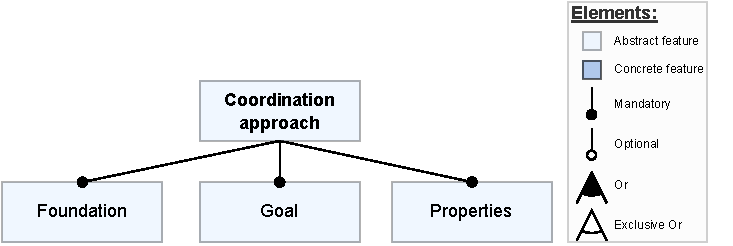
\includegraphics[width=1\textwidth]{images/root}
	\caption{Feature model overview}
	\label{fig: featureModelOverview}
\end{figure}

\subsection{Foundation}

\autoref{fig: foundationFeature} shows the \textbf {Foundation} feature, which consists of \textbf{Syntax}, \textbf{Semantics}, and \textbf{Mechanism}.

\begin{figure}[ht]
	\centering
	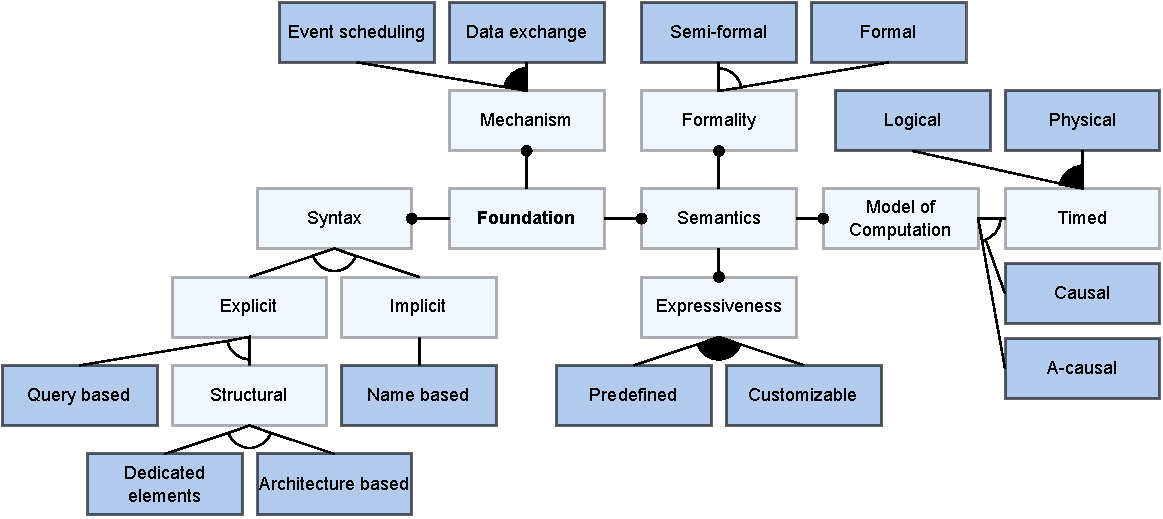
\includegraphics[width=1\textwidth]{images/foundation_feature}
	\caption{Foundation feature}
	\label{fig: foundationFeature}
\end{figure}

\feature{Syntax} The coordination syntax of the elements on which to apply coordination can either be \textit{explicit} or \textit{implicit}.
An implicit syntax is usually based on the names of elements.
For example, one could synchronize the firing of transitions from multiple state machines if they have identical names.

Explicit syntax is either \textit{query based} or \textit{structural}.
% Query-based example
For example, in BCOoL~\cite{varalarsenBCOolBehavioralCoordination2016,varalarsenBehavioralCoordinationOperator2015}, one can write queries to define which elements should coordinate.

A structural definition of coordination uses \textit{dedicated elements} or is \textit{architecture based}.
For example, interactions in BCoorLang are specified by picking dedicated elements that should be coordinated, while coordination in ADLs depends on the architectural configuration~\cite{medvidovicClassificationComparisonFramework2000}, i.e., how ports of systems are connected.

\feature{Mechanism} The main mechanism driving coordination can be \textit{event scheduling}, \textit{data exchange}, or a mix of both.
In the literature, these mechanisms are sometimes called control/event-driven or data-driven, respectively~\cite{papadopoulosCoordinationModelsLanguages1998,varalarsenBCOolBehavioralCoordination2016}.

First, \textit{event scheduling} synchronizes events or imposes a specific event order, i.e., order of state changes in different systems.
Usually, event scheduling is used when systems are given by behavioral models since there might not be a clear concept of an event in a programming language.
For example, in BCOoL~\cite{varalarsenBehavioralCoordinationOperator2015}, one can define relationships between events, such as \textit{happens before} or \textit{synchronize}.

\textit{Data-exchange} means systems communicate by exchanging data.
For example, in the ADL MontiArc~\cite{haberMontiArcArchitecturalModeling2014}, systems send data from the output to the input port.
Data can also be exposed as variables, which are then coupled with variables in other systems, for example, to be the same.
However, data exchange might also happen between systems during the synchronization of events, which is why both coordination mechanisms can be supported simultaneously.

\feature{Semantics} The semantics feature consists of \textit{expressiveness}, \textit{model of computation}, and \textit{formality}.
The expressiveness of coordination can be \textit{predefined}, i.e., a user has a fixed set of coordination mechanisms, for example, a fixed set of connectors with predefined behavior.
Expressiveness is \textit{customizable} if one can define the semantics of coordination, typically by using a dedicated language.
For example, in BCOoL, one can employ the Clock Constraints Specification Language (CCSL)~\cite{andreSyntaxSemanticsClock2009} to define new coordination operators besides the predefined ones~\cite{varalarsenBCOolBehavioralCoordination2016,varalarsenBehavioralCoordinationOperator2015}.

Coordination approaches utilize different \textit{models of computation} (MoC).
A MoC is a set of rules that governs the timed, possibly concurrent execution and coordination of systems~\cite{ptolemaeusSystemDesignModeling2014}.
We categorize MoCs along three types: \textit{timed}, \textit{causal}, \textit{a-causal}.
A \textit{timed} MoC can use \textit{physical} or \textit{logical} time.
% Causal (data)
The categorization of \textit{causal} and \textit{a-causal} MoCs is also present in the co-simulation field~\cite{gomesCoSimulationSurvey2019}.
The causal MoC means that the coordination approach facilitates event and data exchange between different systems such that one system can cause reactions, i.e., state changes in other systems.
For example, a system based on a state machine raises an event, which causes a reaction in a different system.

% A-causal
An a-causal MoC is necessary to deal with related differential equations \cite{lecoentGuaranteedCosimulationCyberphysical2020}.
For example, a variable in one equation should equal a variable in a different equation.
In this case, there is no cause and effect, such as in the causal MoC, but rather, the variables have an a-causal relationship since they should be equal at any time.

% Timed::Logical
\textit{Logical} time means that coordination approaches define when events happen.
Typically, one defines that events take place simultaneously or that one event causes another event immediately or with a fixed delay.
For example, a delay could be 50 milliseconds of logical time, corresponding to time in a simulation that can run arbitrarily fast.

% Timed::Physical
In contrast, \textit{physical} time describes time passing in the physical world.
It is also referred to as \textit{wall-clock} time~\cite{gomesCoSimulationSurvey2019}.
For example, one can define that an event should happen 50 milliseconds after another.
In Lingua Franca~\cite{lohstrohReactorsDeterministicModel2020}, logical time \quotes{chases} physical time, i.e., logical time tries to match the physical time provided by the execution platform.

\textit{Formality} of a coordination approach is either \textit{formal} or \textit{semi-formal}.
Semi-formal approaches are directly implemented in a general-purpose programming language, often with a guiding formalism in mind but without strict adherence to that formalism.

Formal coordination approaches are implemented in a \textit{formal language}, which can then be run on an execution engine implemented for that formalism.
For example, the coordination framework BCoorLang~\cite{krauterBehavioralConsistencyMultimodeling2023} uses graph or term-rewriting as formal languages to coordinate heterogeneous systems in a centralized manner.
It relies on the graph-transformation tool Groove~\cite{rensinkGROOVESimulatorTool2004} or the term-rewriting tool Maude for execution.


\subsection{Goal} % Or even call it motivation
We identified three different \textit{goals} of coordination approaches: \textbf{simulation}, \textbf{execution}, and \textbf{formal validation}, see \autoref{fig: goalFeature}.
A coordination approach can have one or multiple goals, which we will now describe in detail.

\begin{figure}[ht]
	\centering
	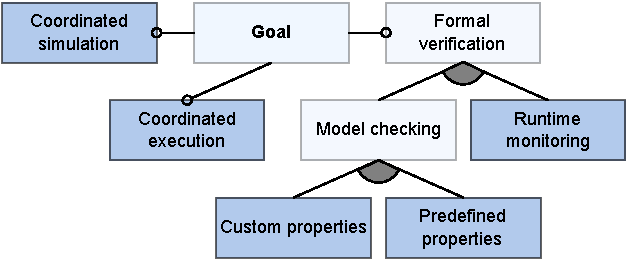
\includegraphics[width=0.7\textwidth]{images/goal_feature}
	\caption{Goal feature}
	\label{fig: goalFeature}
\end{figure}

\feature{Simulation} The most common goal of coordination approaches is a coordinated simulation of multiple systems or behavioral models representing an entire system.
A coordinated simulation is useful because the composition of multiple systems can lead to unexpected behavior, often called \textit{emergent behavior}~\cite{ekerTamingHeterogeneityPtolemy2003}.
Emergent behavior can then be uncovered during simulation before deploying and using the system in a production environment.
Co-simulation approaches such as DACCOSIM~\cite{galtierFMIBasedDistributedMultisimulation2015,dadSynthesisFeedbackDistribution2021} or MECSYCO (Multi-agent Environment for ComplexSYstem CO-simulation)~\cite{camusHybridCosimulationFMUs2016,camusCosimulationCyberphysicalSystems2018} are examples of approaches that have coordinated simulation as their goal.
Simulation is also a goal of coordination frameworks such as BCoorLang~\cite{krauterBehavioralConsistencyMultimodeling2023} and BCOol~\cite{varalarsenBehavioralCoordinationOperator2015}.
Even recent ADLs such as MontiArc~\cite{haberMontiArcArchitecturalModeling2014} provide simulation capabilities.

\feature{Execution} In contrast to only simulation, some coordination approaches aim to provide a coordination infrastructure for system execution upon deployment.
For example, Linda provides a virtual shared memory with read and write operations to coordinate systems.

Furthermore, the recently developed polyglot coordination language \textit{Lingua Franca} provides determinism guarantees during distributed execution~\cite{lohstrohLinguaFrancaDeterministic2021}.
Thus, it eliminates typical coordination concerns faced during coordinating concurrent \textit{execution}.


\feature{Formal validation} Another goal of coordination approaches, especially for safety-critical systems, is formal validation of the coordinated system.

We encountered coordination approaches that validate \textit{predefined properties}, while others support \textit{custom properties}.
% (Definition 5)
For example, the ADL Wright~\cite{allenFormalBasisArchitectural1997} can check \textit{deadlock freedom} of system interactions.
% Darwin and we are checking custom properties: mageeBehaviourAnalysisSoftware1999 krauterBehavioralConsistencyMultimodeling2023
The coordination framework for behavioral consistency~\cite{krauterBehavioralConsistencyMultimodeling2023} supports custom properties written in temporal logic such as Linear Temporal Logic (LTL) and Computational Tree Logic (CTL).

\subsection{Properties}
We identified several reoccurring properties when analyzing coordination approaches.
\autoref{fig: propertiesFeature} depicts the resulting \textit{properties} feature, which we will now explain in detail.

\begin{figure}[ht]
	\centering
	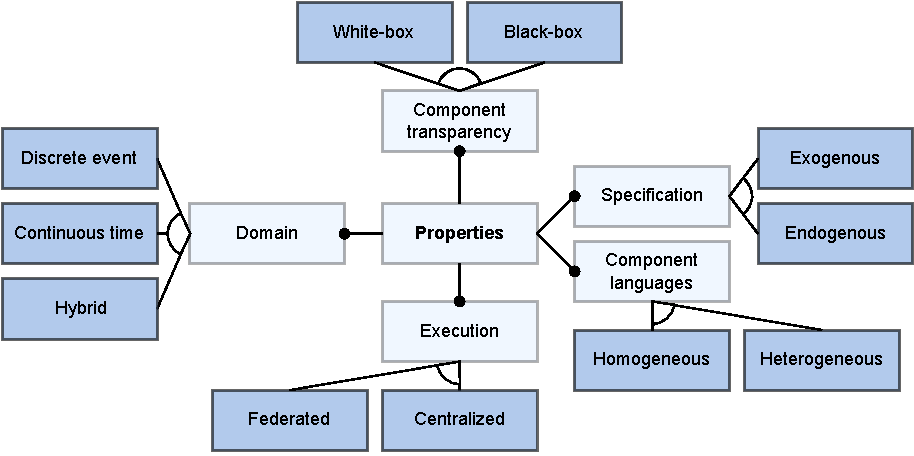
\includegraphics[width=0.9\textwidth]{images/properties_feature}
	\caption{Properties feature}
	\label{fig: propertiesFeature}
\end{figure}

% Maybe add some examples and descriptions here.
\feature{Domain} Coordination approaches operate in different domains like the categorization of co-simulation approaches described in~\cite{gomesCoSimulationSurvey2019,liboniComplexSystemsCosimulation2021}.
First, if a coordination approach is part of the \textit{Discrete Event} (DE) domain, it allows discrete but not continuous state changes~\cite{gomesCoSimulationSurvey2019}.
Typically, coordination frameworks and ADLs operate in the DE domain since variables change their values discontinuously during execution, i.e., immediately change between states.
% discrete = discontinuous

Second, coordination approaches in the \textit{Continuous Time} (CT) domain support systems to have a state that evolves continuously over time.
Often, systems are given by differential equations, which induce continuous variable changes, such as physical systems involving springs and dampeners, see~\cite{gomesCoSimulationSurvey2019}.

Third, the \textit{hybrid} domain is a mix of the DE and CT domains that occur, for example, when simulating cyber-physical systems.
In a hybrid domain, systems should coordinate where some change their state discretely (DE domain) while others evolve continuously over time (CT domain).
% MECSYCO is doing the first, while DACCOSIM is doing the second
Two strategies deal with hybrid systems: either adapt the systems from the CT to the DE domain or vice versa~\cite{gomesCoSimulationSurvey2019}.

\feature{System transparency} Some coordination approaches require constituent systems to be entirely transparent (\textit{white-box}), while others only require a fixed interface (\textit{black-box}).
Usually, black-box approaches are needed to protect \textit{intellectual property} (IP) when different companies want to work together without sharing all the details concerning their systems.

For example, DACCOSIM only requires each system to conform to the FMI specification for Co-Simulation.

\feature{Specification} We distinguish between \textit{endogenous} and \textit{exogenous} specification of coordination, as described for coordination languages in~\cite{arbabWhatYouMean1998}.
For example, when using the coordination language Linda~\cite{carrieroLindaContext1989}, one uses coordination-specific operations such as \textsf{out} and \textsf{in} inside system programs to write to and read from the shared tuple space, respectively.
Thus, Linda is \textit{endogenous} since one has to modify the behavior of the systems to add coordination.

On the other hand, \textit{exogenous} coordination approaches keep coordination aspects outside of systems.
However, systems must still be created with coordination in mind to expose possible coordination points.
For example, BCOol~\cite{varalarsenBehavioralCoordinationOperator2015} uses language behavioral interfaces to define events, which can then be used to specify \textit{exogenous} coordination rules outside the systems.
Endogenous coordination approaches tend to mix computation and coordination~\cite{arbabWhatYouMean1998}.

\feature{System languages} Coordination approaches typically only support \textit{homogeneous} systems.
For example, coordination languages, such as Lingua Franca~\cite{lohstrohReactorsDeterministicModel2020}, currently only support coordination if each system is given in the same programming language.

However, coordination frameworks allow \textit{heterogeneous} systems, i.e., systems specified in different behavioral modeling languages.
For example, BCoorLang~\cite{krauterBehavioralConsistencyMultimodeling2023} supports all modeling languages that one can describe using rewriting semantics.

\feature{Execution} A coordination approach is realized using either a \textit{centralized} or \textit{federated} execution.
In a \textit{centralized} execution, all systems are executed by one engine, which enforces coordination.
For example, BCoorLang composes the behavior of all system specifications into a global behavior specification, which is then executed by a graph transformation or term-rewriting tool.

On the other hand, in a \textit{federated execution}, systems run independently and only coordinate using a shared infrastructure through predefined connections.
Federated execution can still happen on the same physical machine, i.e., it does not mean that systems must be \textit{distributed} across different physical machines. 

For example, the coordination language Lingua Franca~\cite{lohstrohReactorsDeterministicModel2020} supports federated execution on one machine by providing a runtime infrastructure.
DACCOSIM~\cite{galtierFMIBasedDistributedMultisimulation2015} goes one step further and allows a \textit{distributed} federated execution.


\section{Application of the feature model} \label{sec: application}
\autoref{tab:classification} shows the application of our feature model to four different coordination approaches.
Each approach comes from a different category: co-simulation (\textit{DACCOSIM}~\cite{galtierFMIBasedDistributedMultisimulation2015,dadSynthesisFeedbackDistribution2021}), coordination language (\textit{Linda}~\cite{carrieroLindaContext1989,carrieroLindaAlternativeMessagepassing1994}), ADL (\textit{MontiArc}~\cite{haberMontiArcArchitecturalModeling2014}), and coordination framework (\textit{BCoorLang}~\cite{krauterBehavioralConsistencyHeterogeneous2021,krauterBehavioralConsistencyMultimodeling2023}).

\begin{table}
	\centering
	\caption{Approach classification}
	\label{tab:classification}
	\resizebox{\textwidth}{!}{
	\SetTblrInner{colsep=2pt}
	\begin{tblr}{
			column{2-Z} = {c},
			hline{1, 2, Z} = {-}{1.2pt, solid}, % Z is the last row/column
			hline{8, 12} = {-}{dashed},
			vline{2-Y} = {2-Z}{solid},
		}
		\diagbox[linewidth=1.1pt,font=\bfseries]{Feature}{Approach} & \textbf{DACCOSIM} & \textbf{Linda} & \textbf{MontiArc} & \textbf{BCoorLang} \\
		
		\textbf{Foundation} \\
		\hspace{1mm} Syntax & Architecture based & Name based & Architecture based & Dedicated elements \\
		\hspace{1mm} Mechanism & Data-Exchange & Data-Exchange & Data-Exchange & Event-Scheduling \\
		\hspace{1mm} Expressiveness & Predefined & Predefined & Predefined & Predefined \\
		\hspace{1mm} MoC & Causal & Causal & Logical, Causal & Logical \\
		\hspace{1mm} Formality & Semi-formal & Semi-formal & Semi-formal & Formal \\
		
		\textbf{Goal} \\
		\hspace{1mm} Simulation & + & - & + & + \\
		\hspace{1mm} Execution & - & + & - & - \\
		\hspace{1mm} Formal verification & - & - & - & Custom properties \\
		
		\textbf{Properties} \\
		\hspace{1mm} Domain & Hybrid & Discrete event & Discrete event & Discrete event \\
		\hspace{1mm} Comp. transparency & Black-box & White-box & White-box & White-box \\
		\hspace{1mm} Specification & Exogenous & Endogenous & Endogenous & Exogenous \\
		\hspace{1mm} Comp. languages & Homogeneous & Homogeneous & Homogeneous & Heterogeneous \\
		\hspace{1mm} Execution & Federated & Federated & Centralized & Centralized \\
	\end{tblr}
	}
\end{table}

In addition, we classified the following approaches: Ptolemy~\cite{ekerTamingHeterogeneityPtolemy2003,ptolemaeusSystemDesignModeling2014}, Wright \cite{allenFormalBasisArchitectural1997,allenFormalApproachSoftware1997}, CommUnity~\cite{fiadeiroSemanticsArchitecturalConnectors1997,oliveiraCommUnityWorkbench2007}, Metropolis~\cite{balarinMetropolisIntegratedElectronic2003}, UMoC\texttt{++}~\cite{mathaikuttyUMoCBasedMultiMoC2006}, Lingua Franca~\cite{lohstrohReactorsDeterministicModel2020,lohstrohLinguaFrancaDeterministic2021}, Reo~\cite{arbabReoChannelbasedCoordination2004}, BIP~\cite{bliudzeAlgebraConnectorsStructuring2008,basuRigorousComponentBasedSystem2011},
MECSYCO~\cite{camusCosimulationCyberphysicalSystems2018,camusHybridCosimulationFMUs2016},
CoSim20~\cite{liboniComplexSystemsCosimulation2021},
BCOoL~\cite{varalarsenBehavioralCoordinationOperator2015,varalarsenBCOolBehavioralCoordination2016},
Manifold~\cite{arbabOverviewManifoldIts1993,papadopoulosModellingActivitiesInformation1998}, and ForSyDe~\cite{sanderSystemModelingTransformational2004,sanderForSyDeSystemDesign2016}.
Due to space constraints, we cannot show all classifications, but the full data set is available in the artifacts of this paper~\cite{timkrauterArtifactsCoordination2024}.

In \autoref{fig: venns}, we compare BCoorLang and MontiArc with Linda on the left and DACCOSIM on the right.
The figure shows Venn diagrams comparing the feature sets of each approach, where each colored part states which features are contained.
In addition, the number in each area states the amount of contained features.

For example, when looking at the Venn diagram on the left in \autoref{fig: venns}, the \textsf{1} in the circle part at the bottom describes that MontiArc has one \textit{original} feature, while the \textsf{3} in the intersection of all approaches in the middle declares that they all have three features in \textit{common}, see \autoref{tab:classification}.

\begin{figure}[ht]
	\centering
	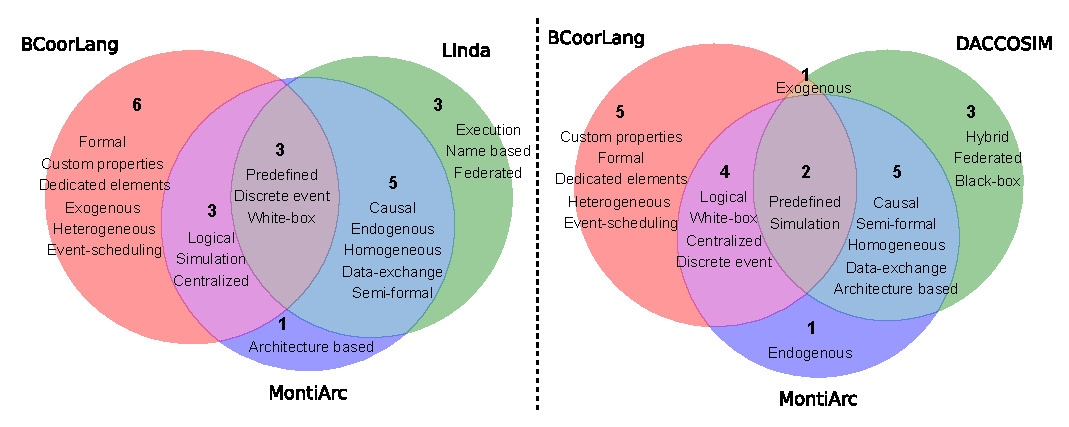
\includegraphics[width=1\textwidth]{images/venns}
	\caption{Feature comparison: BCoorLang, MontiArc, and Linda/DACCOSIM}
	\label{fig: venns}
\end{figure}

The Venn diagram on the left in \autoref{fig: venns} shows that Linda has three original features compared to BCoorLang and MontiArc:
execution as goal, a name-based syntax, and a federated execution.
Furthermore, one can see that coordination frameworks, i.e., BCoorLang (the diagram is similar for BCOol~\cite{varalarsenBehavioralCoordinationOperator2015,varalarsenBCOolBehavioralCoordination2016}) greatly differ from ADLs and coordination languages.
Coordination frameworks have multiple original features, such as supporting heterogeneous system languages and formal validation using custom properties.

Similarly, on the right in \autoref{fig: venns}, BCoorLang and MontiArc are compared with the co-simulation approach DACCOSIM.
One can see that BCoorLang and DACCOSIM do not have many features in common, probably due to their different goals as a coordination approach.
Co-simulation approaches like DACCOSIM have original features, such as a federated execution, hybrid domain, and black-box system transparency.

Venn diagrams give a good approximation of the similarity between three specific coordination approaches.
However, they do not tell the whole story since each feature is given equal weight, which is not always adequate.
For example, a difference in the \textit{domain} feature is more profound than most other differences.
We stick to this simple weighting throughout this paper since the importance of features can be subjective.
However, one can adapt the analysis using the provided data and scripts~\cite{timkrauterArtifactsCoordination2024}.

\section{Findings} \label{sec: findings}

This section describes the findings of applying our taxonomy to the different coordination approaches.
We start by summarizing the common features of each coordination category before stating the general insights we have attained.
In addition, we cluster the approaches based on their feature similarity and discuss the results.

\subsection{Common features}

% Highlight typical features for ADLs, Coordination language, Co-simulation, and coordination frameworks.
% ADL
\textbf{ADLs} primarily have \textit{simulation} as their goal, while a small subset allows predefined properties to be verified.
As expected, the coordination syntax of all ADLs is architecture-based, using components with ports and connectors between them.
All ADLs operate in the discrete event domain.
Furthermore, components in ADLs are white-box and homogeneous, and coordination specification is usually exogenous, i.e., part of the connectors.
An exception is MontiArc, where ports can be marked as \textit{synchronized} only allowing synchronous interactions through a port; that is, the coordination specification is endogenous and partly present inside components.

% Coordination language
\textbf{Coordination languages} can have simulation and execution as their goal while operating in the discrete event domain.
Furthermore, coordination syntax is also most likely architecture-based, i.e., the idea of subsystems, ports, and connectors/channels between them is also used in most coordination languages.
In addition, the systems in coordination languages are white-box and homogeneous but have both endogenous and exogenous coordination specifications.
Notably, some coordination languages offer a federated execution not supported by ADLs.

% Co-Simulation
As the name suggests, all \textbf{co-simulation} approaches have merely simulation as their goal.
Similar to ADLs and coordination languages, coordination syntax is architecture-based.
However, compared to the other categories, they operate in the hybrid domain, facilitating data exchange between black-box systems.
The systems can be homogeneous or heterogeneous by wrapping them in specific formalisms such as DEVS in the case of MECSYCO.
Typically, execution is federated, while some approaches, such as DACCOSIM, even allow for a distributed execution.

% Coordination frameworks
\textbf{Coordination frameworks} have simulation and formal validation as their goal.
Coordination syntax is diverse but usually uses event scheduling in the discrete event domain.
Furthermore, coordination specification is exogenous to support heterogeneous systems, which are white-box.
In contrast to coordination languages and co-simulation approaches, execution is centralized.
In addition, some coordination frameworks, such as BCoorLang, facilitate formal verification of custom properties, which is a rare feature.

% High-level insights/findings
\subsection{General insights}

\textbf{Architecture-based coordination syntax is widely used.}
Remarkably, coordination approaches from all categories use concepts such as components, ports, and connectors to express coordination.
%The specific coordination details vary between different approaches, but there appears to be broad consensus on the importance of clearly representing the system architecture for effective coordination.
The precise coordination details may differ across various approaches, but there seems to be a general consensus regarding the significance of accurately representing the system architecture for efficient coordination.

\textbf{Formal verification is rarely supported.}
Most of the studied coordination approaches have simulation as their goal, while formal verification is uncommon.
This could be attributed to the problem of formally representing heterogeneous systems engaged in coordination and the rapid growth of state spaces when multiple systems are involved.

\textbf{Coordination frameworks do not support Data-Exchange.}
All coordination frameworks %besides Ptolemy 
support \textit{event-scheduling} but not \textit{data-exchange} as a coordination mechanism.
%This is likely because data exchange is difficult when heterogeneous systems are present.
%However, data exchange is omnipotent in real-world systems, so it is the main coordination mechanism used in co-simulation approaches and coordination languages.
This difficulty likely arises due to the presence of heterogeneous systems, making data exchange challenging.
Nevertheless, data exchange is omnipotent in real-world systems, serving as the primary coordination mechanism utilized in co-simulation methods and coordination languages.
%Thus, for coordination frameworks to be employed in real-world scenarios, they must support data exchange.
Therefore, coordination frameworks must possess the capability to facilitate data exchange to be effectively utilized in real-world scenarios.

\subsection{Feature clustering analysis}

We further analyze the classification of the approaches mentioned in \autoref{sec: application} to determine how they compare across and inside the four categories.
We clustered the approaches to see similarities and differences by just looking at the feature data of each approach, without considering to which category they belong.
The data and scripts to reproduce our analysis are available in~\cite{timkrauterArtifactsCoordination2024}.
We apply a standard clustering algorithm using Jaccard distance to measure the similarity of the feature sets.
Jaccard distance is the one-complement of Jaccard similarity for two sets, defined as the ratio of their intersection to their union~\cite{levandowskyDistanceSets1971}.
It is a widely used and reasonable dissimilarity measure for sets~\cite{levandowskyDistanceSets1971}.

\autoref{fig: clusters} shows a scatter plot with approximate positions of each approach derived solely from the distances between them.
It provides a bird's-eye view of the similarity or dissimilarity between all the studied coordination approaches---this is in contrast to the previous Venn diagrams, which only compare three approaches.
Furthermore, it highlights the clustering results by coloring each data point.
We selected clustering parameters to reduce the number of unclustered approaches while ensuring that we do not consolidate everything into just one cluster.

\begin{figure}[ht]
	\centering
	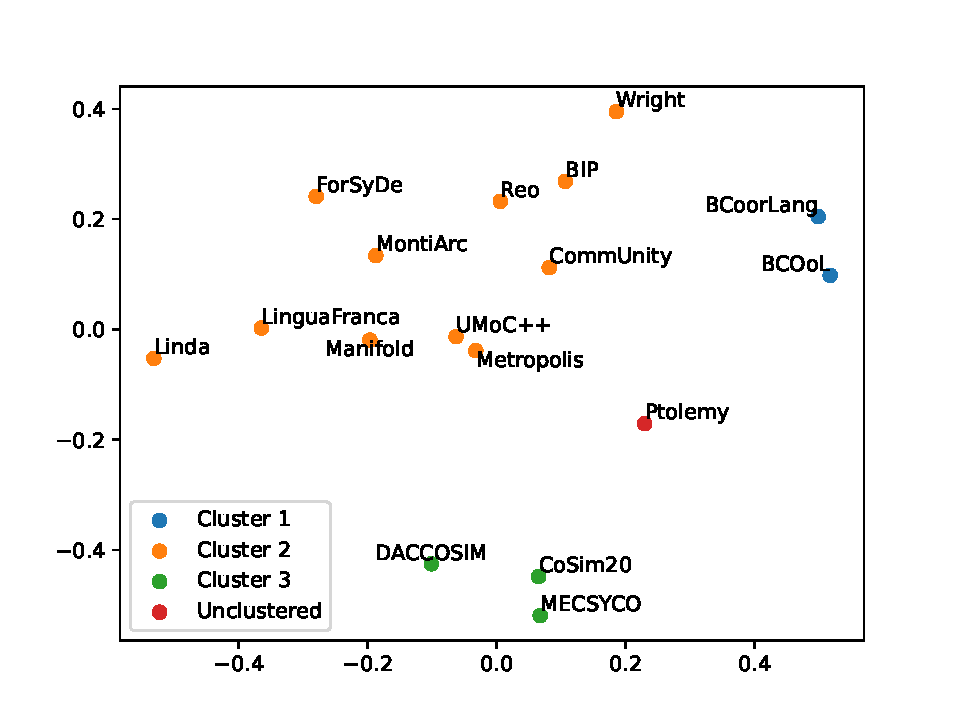
\includegraphics[width=1\textwidth]{images/approach_scatter}
	\caption{Feature distance and clustering of approaches}
	\label{fig: clusters}
\end{figure}

% Description of the plot
The clustering algorithm finds three clusters, including all but one approach.
\textbf{Cluster 1} contains only the coordination frameworks BCoorLang and BCOol, 
while \textbf{cluster 2} consists of a mix of coordination languages and ADLs, such as Linda and Lingua Franca, as well as Wright and MontiArc, respectively.
\textbf{Cluster 3} includes three co-simulation approaches, but no cluster contains Ptolemy.

% Interpretation of the plot
We interpret cluster 1 as representing the coordination framework category.
Similarly, cluster 3 is the co-simulation cluster, showing that according to our taxonomy, co-simulation approaches are similar and have original features not found in the other categories.
Cluster 2 contains coordination languages and ADLs.
Even if the maximum distance between approaches is reduced to be considered part of the same cluster (clustering parameter), one cannot separate the approaches into two categories.
Thus, we conclude that coordination languages and ADLs have more similarities in features compared to, for instance, co-simulation approaches or coordination frameworks.

As the only approach, Ptolemy remains unclustered. 
Although we would classify Ptolemy as a coordination framework, it includes features from all categories and is not part of any cluster.
%It is fascinating that one approach can offer such diverse features.
It is intriguing how a single approach like Ptolemy may encompass a wide variety of features.

\section{Conclusion \& future work} \label{sec: conclusion}

% Summary and Contributions
% Feature model/taxonomy --> link back to motivation
The main contribution of this paper is a taxonomy of coordination approaches represented as a feature model.
This taxonomy facilitates the categorization and comparison of approaches across previously isolated categories.
Consequently, we provide a comprehensive overview of coordination in the literature and the state of the art.
% Application and data set
Furthermore, we apply our taxonomy to 17 coordination approaches and publish the results as open data \cite{timkrauterArtifactsCoordination2024}.
% Findings
Analyzing the resulting data, we identify characteristic features in each category, provide overarching insights, and cluster the approaches regarding their similarity. 

% Future work
In future work, we aim to refine our taxonomy further and apply it to more approaches to obtain an even more comprehensive overview of coordination approaches.

\bibliographystyle{splncs04}
\bibliography{bib}

\end{document}
